\documentclass[a4paper]{article}
\usepackage[utf8]{inputenc}




\title{Pendolo reversibile - Caduta libera\\ analisi dei dati}
\author{Ali Matteo,\\Broggi Diana, Cantarini Giulia}
\date{ }

\usepackage{tabularx}
\usepackage{natbib}
%\usepackage[demo]{graphicx}
\usepackage{graphicx}

%\usepackage[margin=1.0in]{geometry}

\usepackage{tikz}

\usepackage{subcaption}
\usepackage{caption}
\usepackage{amsmath, amsthm}

\usepackage{mathrsfs}

\usepackage{pgfplots}

\usepackage{caption}



%\pgfplotsset{width=4cm,compat=1.9}

\theoremstyle{definition}
\newtheorem{rich}{richiamo matematico}[section]





%roba che crea comando per centrare immagine dentro immagine piu grande
%https://tex.stackexchange.com/a/308286
\newlength{\imagew}
\newlength{\imageh}
\newlength{\legendw}
\newlength{\legendh}
\newlength{\legendx}
\newlength{\legendy}
\newcommand{\graphicswithlegend}[6]{
	\setlength{\imagew}{#1}
	\settoheight{\imageh}{\includegraphics[width=\imagew]{#2}}
	
	\setlength{\legendw}{#3\imagew}
	\settoheight{\legendh}{\includegraphics[width=\legendw]{#4}}
	
	\setlength{\legendx}{\imagew}
	\addtolength{\legendx}{-\legendw}
	\addtolength{\legendx}{-#5\imagew}
	
	\setlength{\legendy}{\imageh}
	\addtolength{\legendy}{-\legendh}
	\addtolength{\legendy}{-#6\imageh}
	
	\includegraphics[width=\imagew]{#2}%
	\llap{
		\hspace{-\the\legendx}
		\raisebox{\legendy}{\includegraphics[width=\legendw]{#4}}
		\hspace{\the\legendx}
	}
}



\begin{document}
	\pagenumbering{arabic}
	\maketitle
	\section*{Pendolo reversibile di Kater}
	La posizione di \(m_{A}\) è stata tenuta costante:
	\begin{figure}[!htbp]
		\captionsetup{labelformat=empty}
		\caption{distanza di \(m_{A}\) dal coltello 2 in metri}
		\makebox[1 \textwidth][c]{       %centering table
			\begin{tabular}{ccccc}
				\hline
				\hline
				0.159 &0.16 & 0.159 &0.159& 0.16\\

				\hline
				\hline
			\end{tabular}
		}
	\end{figure}


		 \noindent Riportiamo le diverse distanze di \(m_{B}\) dal coltello 2 in metri, e i relativi periodi
		\makebox[\textwidth]{
			{
				\normalsize
				in secondi:
			}
		}
	
	\noindent distanza 1:	
	\begin{table}[!ht]
		\centering
		\input{relazione_Pendolo_Kater/tabelle/tableDistances1.tex}
	\end{table}
	
	
	\begin{figure}[!htbp]
		\makebox[1 \textwidth][c]{       %centering table
			\begin{tabular}{l|*{11}{c}}
				\hline
				\hline
				Periodo 1 & 1.9485 & 1.9483 & 1.9488 & 1.9489 & 1.9483 & 1.9484 & 1.9487 & 1.9487 & 1.9482 & \\
				\hline
				\hline
				Periodo 2 & 1.8306 & 1.83 & 1.8295 & 1.8286 & 1.8292 & 1.8298 & 1.8288 & 1.8287 & 1.829 & 1.8289\\
				\hline
				\hline
			\end{tabular}
			
		} %close centering
	\end{figure}
	
	\noindent distanza 2:
	\begin{table}[!ht]
		\centering
		\input{relazione_Pendolo_Kater/tabelle/tableDistances2.tex}
	\end{table}
	
	\begin{figure}[!htbp]
		\makebox[1 \textwidth][c]{ 
			\begin{tabular}{l|*{11}{c}}
				\hline
				\hline
				Periodo1 & 1.9637 & 1.9638 & 1.9636 & 1.9636 & 1.9635 & 1.9633 & 1.9632 & 1.963 & 1.9634 & \\
				\hline
				Periodo2 & 1.8614 & 1.8612 & 1.861 & 1.8612 & 1.8608 & 1.8606 & 1.8608 & 1.8611 & 1.8612 & 1.8612 & \\
				\hline
				\hline	
			\end{tabular}
		} %close centering
	\end{figure}
	
	\noindent distanza 3:
	\begin{table}[!ht]
		\centering
		\input{relazione_Pendolo_Kater/tabelle/tableDistances3.tex}
	\end{table}
	
	
	\begin{figure}[!htbp]
		\makebox[1 \textwidth][c]{ 
			\begin{tabular}{l|*{11}{c}}
				\hline
				\hline
				Periodo1 & 1.9827 & 1.9824 & 1.9826 & 1.9822 & 1.9828 & 1.9825 & 1.9826 & 1.9828 & 1.9825 & \\
				\hline
				Periodo2 & 1.9264 & 1.9274 & 1.9264 & 1.9263 & 1.927 & 1.9258 & 1.9258 & 1.9257 & 1.9271 & 1.927 & \\
				\hline
				\hline
			\end{tabular}
		} %close centering
	\end{figure}
	.\\\\
	\noindent distanza 4:
	\begin{table}[!ht]
		\centering
		\input{relazione_Pendolo_Kater/tabelle/tableDistances4.tex}
	\end{table}
	
	
	\begin{figure}[!htbp]
		\makebox[1 \textwidth][c]{ 
			\begin{tabular}{l|*{11}{c}}
				\hline
				\hline
				Periodo1 & 1.9884 & 1.9887 & 1.9879 & 1.9877 & 1.9877 & 1.9876 & 1.9876 & 1.9876 & 1.988 & \\
				\hline
				Periodo2 & 1.9378 & 1.9381 & 1.9369 & 1.9379 & 1.9366 & 1.9386 & 1.9374 & 1.9357 & 1.9357 & 1.9367 & \\
				\hline
				\hline
			\end{tabular}
		} %close centering
	\end{figure}

	\noindent distanza 5:
	
	\begin{table}[!htbp]
		\centering
		\input{relazione_Pendolo_Kater/tabelle/tableDistances5.tex}
	\end{table}
	
	
	\begin{figure}[!htbp]
		\makebox[1 \textwidth][c]{ 
			\begin{tabular}{l|*{11}{c}}
				\hline
				\hline
				Periodo1 & 2.0279 & 2.0265 & 2.0271 & 2.0256 & 2.0244 & 2.0251 & 2.0241 & 2.0232 & 2.0226 & 2.0226 & \\
				\hline
				Periodo2 & 2.0075 & 2.0074 & 2.0071 & 2.0061 & 2.0065 & 2.0063 & 2.0065 & 2.0061 & 2.0061 & \\
				\hline
				\hline
			\end{tabular}
		} %close centering
	\end{figure}

	\noindent distanza 6:
	\begin{table}[!ht]
		\centering
		\input{relazione_Pendolo_Kater/tabelle/tableDistances6.tex}
	\end{table}
	
	
	\begin{figure}[!htbp]
		\makebox[1 \textwidth][c]{ 
			\begin{tabular}{l|*{11}{c}}
				\hline
				\hline
				Periodo1 & 2.0227 & 2.0222 & 2.0221 & 2.0228 & 2.0221 & 2.0217 & 2.0218 & 2.0217 & 2.0217 & \\
				\hline
				Periodo2 & 2.1072 & 2.1046 & 2.1035 & 2.1046 & 2.1032 & 2.1034 & 2.1043 & 2.1025 & 2.1039 & 2.1024 & \\
				\hline
				\hline
			\end{tabular}
			
		} %close centering
	\end{figure}
	\begin{figure}[!htbp]
				\captionsetup{labelformat=empty}
		\caption{dist \(m_{A}\)= 0.159 metri}
	\makebox[1 \textwidth][c]{ 
		\begin{tabular}{c|cc}
			\hline
			\hline
			dist \(m_{B}\) (m) & Periodo 1 (s) & Perido 2 (s)\\
			\hline
			1: 0.2940 &1.949 &1.82931 \\
			2: 0.2350& 1.963 &1.86105\\
			3: 0.1682& 1.983&  1.92649\\
			4: 0.1584&  1.988&  1.93714 \\
			5: 0.1024 &  2.007 &2.02491 \\
			6: 0.0628 & 2.022 &2.10396\\
			\hline
			\hline
		\end{tabular}
		
	} %close centering
\end{figure}
.\\\\\\\\\\\\
	\begin{figure}[!ht]
	\makebox[1 \textwidth][c]{       %centering table
		\resizebox{0.90 \textwidth}{!}{   %resize table
			\includegraphics{relazione_Pendolo_Kater/computed_data/punti.png}
		} %close resize
	} %close centering

\end{figure}

\subsection*{calcolo di g}

\noindent Selezioniamo la distanza 4 e la distanza 5 per il calcolo di \(T^{*}\):

\[T^{*} = \frac{T_{2}(x_{4})T_{1}(x_{5})-T_{1}(x_{4})T_{2}(x_{5})}{T_{1}(x_{5})-T_{2}(x_{5})-T_{1}(x_{4})+T_{2}(x_{4})}\]
\makebox[\textwidth]{
	{
		\small
		\(\sigma_{T^{*}} = \sqrt{\left ( \frac{\partial T^{*}}{\partial T_{2}(x_{4})} \right )^{2}\sigma_{T2(x4)}^{2} + \left ( \frac{\partial T^{*}}{\partial T_{2}(x_{5})} \right )^{2} \sigma_{T2(x5)}^{2}+\left ( \frac{\partial T^{*}}{\partial T_{1}(x_{4})} \right )^{2} \sigma_{T1(x4)}^{2}+\left ( \frac{\partial T^{*}}{\partial T_{1}(x_{5})} \right )^{2} \sigma_{T1(x5)}^{2}}\)
	}
}
\[\rightarrow \quad T*=2.0017 \pm 0.0002 s\]
attraverso questo risultato abbiamo calcolato una prima stima di g:
\[g = \frac{4\pi ^{2}D}{(T^{*})^{2}} \qquad \sigma _{g} = \frac{4\pi ^{2}D}{(T^{*})^{3}}\sigma _{T}\]
\[g = 9.794 \pm 0.002 m/s^{2}\]
\noindent \(t= \frac{\left | g_{osservata} - g_{attesa} \right |}{\sigma_{g}} = 4\), un valore di t sopra al 2 indica che la stima da noi raggiunta è probabilmente affetta da errori sistematici.\\

\subsection*{stima dell'errore sistematico}
\noindent Correzione di \(T^{*}\) per angoli di oscillazione finiti: \(T^{*}_{1} = 2\pi \sqrt{\frac{D}{g}}(1+\frac{\theta ^{2}}{16})\) con \(\theta = 0.0861 \pm 0.0008 rad\).\\
\[g_{1}= \frac{4\pi ^{2}D}{T^{*2}}\left ( 1+\frac{\theta ^{2}}{16} \right )^{2} \pm \sqrt{\left ( \frac{\partial g}{\partial T} \right )^{2}\sigma _{T}^{2}+\left ( \frac{\partial g}{\partial \theta }\right )^{2}\sigma _{\theta }^{2} }=9.803\pm0.002 m/s^{2}\]
\(t= \frac{\left | g_{1 osservata} - g_{attesa} \right |}{\sigma_{g}} = \frac{\left | 9.803 - 9.807 \right |}{0.002} = 2\), il confronto con g attesa porta a un risultato migliore del precedente.\\
\noindent L'errore sistematico sulla prima misura di g era pari a \( \left | g-g_{1} \right | =  0.009 m/s^{2}\), dello stesso ordine di grandezza di quello casuale \(\rightarrow\) non trascurabile.\\\\
L'errore sistematico su \(g_{1}\) sarà meno notevole:
\[ T^{*}_{2}= 2\pi \sqrt{\frac{D}{g}} \left (1+\frac{\theta ^{2}}{16}+\frac{9\theta ^{4}}{1024}+\frac{25\theta ^{6}}{16384} \right )\] 
 \( \sigma_{g1}=\left | g_{2}-g_{1} \right | =  9 \cdot 10^{-6} m/s^{2}\) è l'errore sistematico sulla stima di \(g_{1}\), trascurabile rispetto a quello casuale.  Non prevediamo di aver commesso altri errori sistematici rilevanti, concludiamo che la nostra stima per l'accelerazione di gravità è \(g = g_{1} = 9.803 \pm 0.002 m/s^{2}\).
\section*{Caduta libera}
	Riportiamo le diverse altezze,in metri, da cui abbiamo fatto cadere la pallina ed i relativi tempi di caduta in secondi:\\
	
	\noindent altezza 1:
	
\begin{table}[!htbp]
	\centering
	\input{relazione_caduta_libera/tabelle/tableHeights1.tex}
\end{table}

\begin{table}[!htbp]
	\centering
	\input{relazione_caduta_libera/tabelle/tableTimes1.tex}
\end{table}

	\noindent altezza 2:
	
\begin{table}[!htbp]
	\centering
	\input{relazione_caduta_libera/tabelle/tableHeights2.tex}
\end{table}

\begin{table}[!htbp]
	\centering
	\input{relazione_caduta_libera/tabelle/tableTimes2.tex}
\end{table}
	\noindent altezza 3:
		
\begin{table}[!htbp]
	\centering
	\input{relazione_caduta_libera/tabelle/tableHeights3.tex}
\end{table}
\begin{table}[!htbp]
	\centering
	\input{relazione_caduta_libera/tabelle/tableTimes3.tex}
\end{table}
.\\\\\\\\\\\\\\
	\noindent altezza 4:
		
\begin{table}[!htbp]
	\centering
	\input{relazione_caduta_libera/tabelle/tableHeights4.tex}
\end{table}
\begin{table}[!htbp]
	\centering
	\input{relazione_caduta_libera/tabelle/tableTimes4.tex}
\end{table}

	\noindent altezza 5:	
	
\begin{table}[!htbp]
	\centering
	\input{relazione_caduta_libera/tabelle/tableHeights5.tex}
\end{table}
\begin{table}[!htbp]
	\centering
	\input{relazione_caduta_libera/tabelle/tableTimes5.tex}
\end{table}
	
	\noindent altezza 6:\\	
	
\begin{table}[!htbp]
	\centering
	\input{relazione_caduta_libera/tabelle/tableHeights6.tex}
\end{table}
\begin{table}[!htbp]
	\centering
	\input{relazione_caduta_libera/tabelle/tableTimes6.tex}
\end{table}


	
\begin{figure}[!htbp]
	\captionsetup{labelformat=empty}
	\caption{Tabella1}
	\makebox[1 \textwidth][c]{ 
		\begin{tabular}{c|c}
			\hline
			\hline
			altezza (m) & tempo di caduta (s)\\
			\hline
			1: \(0.603 \pm 0.0003\) &\(0.315 \pm 0.002\)\\
			2:  \(0.584 \pm  0.0003\)& \(0.309 \pm  0.002\)\\
			3:  \(0.557 \pm 0.0004\)& \( 0.295 \pm  0.003\)\\
			4: \(0.505 \pm  0.0003\)& \( 0.287 \pm  0.002\)\\
			5:\( 0.451 \pm 0.0003\)&  \(0.270 \pm 0.002\)\\
			6: \(0.396 \pm  0.0005\) &\(0.248 \pm   0.002\)\\
			\hline
			\hline
		\end{tabular}
	} %close centering
\end{figure}

.\\\\\\\\\\\\\\\\\\\\\\
\begin{figure}[!ht]
	\makebox[1 \textwidth][c]{       %centering table
		\resizebox{0.90 \textwidth}{!}{   %resize table
			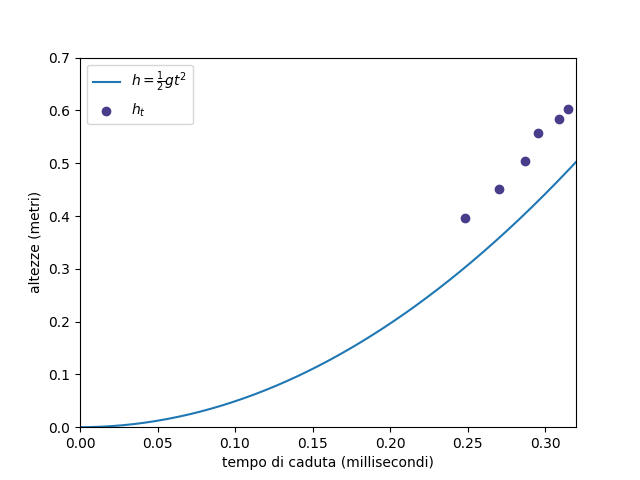
\includegraphics{relazione_caduta_libera/computed_data/parabola.png}
		} %close resize
	} %close centering
	
\end{figure}

\begin{figure}[!htbp]
	\captionsetup{labelformat=empty}
	\caption{Tabella2.a}
	\makebox[1 \textwidth][c]{ 
		\begin{tabular}{c|c}
			\hline
			\hline
			x: altezza (m) & y: tempo di caduta\(^{2}\) (\(s^{2}\))\\
			\hline
			1: \(0.603 \pm 0.0003\) &\(0.099\pm 0.001\)\\
			2:  \(0.584 \pm  0.0003\)& \(0.096 \pm 0.001\)\\
			3:  \(0.557 \pm 0.0004\)& \(  0.087 \pm 0.002 \)\\
			4: \(0.505 \pm  0.0003\)& \(  0.083 \pm  0.001 \)\\
			5: \( 0.451 \pm 0.0003\)&  \( 0.073 \pm  0.001\)\\
			6: \(0.396 \pm  0.0005\) &\(0.062 \pm  0.001\)\\
			\hline
			\hline
		\end{tabular}
	} %close centering
	\caption{\(\sigma_{t^{2}} = 2t\sigma_{t}\)}
\end{figure}

\noindent Abbiamo eseguito l'interpolazione lineare dei dati in Tabella2.a con il metodo dei minimi quadrati pesati(i pesi utilizzati sono \( w_{i} = \frac{1}{\sigma_{ti}^{2}}\) poichè \(\sigma_{ti} >> \sigma_{hi}\) ) 
\[\Delta = \sum (w_{i}y_{i}^{2})\sum w_{i}-(\sum w_{i}y_{i})^{2}\]
\[B = \frac{\sum w_{i}\sum w_{i}x_{i}y_{i}-\sum w_{i}x_{i}\sum w_{i}y_{i}}{\Delta } \pm \sqrt{\frac{\sum w_{i}}{\Delta }} =0.17 \pm 0.006 m/s^{2}\]
\[A = \frac{\sum w_{i}x_{i}^{2}\sum w_{i}y_{i}-\sum w_{i}x_{i}\sum w_{i}x_{i}y_{i}}{\Delta } \pm \sqrt{\frac{w_{i}x_{i}^{2}}{\Delta }} = -0.008 \pm 0.003 s^{2}\]

.\\\\\\\\\\\\
\begin{figure}[!ht]
	\captionsetup{labelformat=empty}
	\makebox[1 \textwidth][c]{       %centering table
		\resizebox{0.90 \textwidth}{!}{   %resize table
			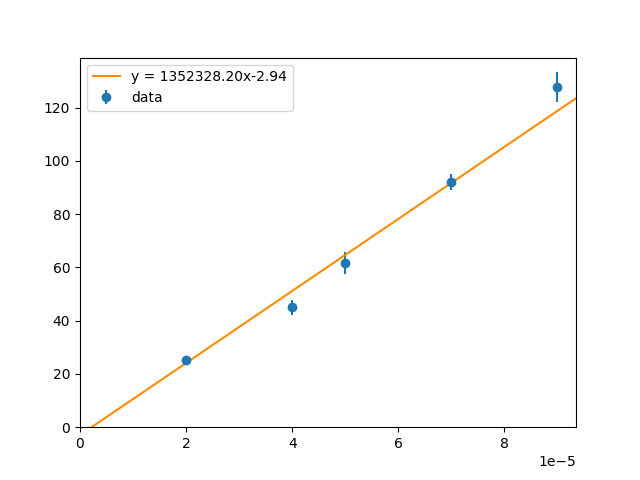
\includegraphics{relazione_caduta_libera/computed_data/retta.png}
		} %close resize
	} %close centering
\end{figure}

\noindent Infine, abbiamo calcolato l'accelerazione di gravità con \(g = \frac{2}{B} \pm \frac{2}{B^{2}}\sigma_{B} = \) \\\(=11.3 \pm 0.4 m/s^{2}\).
\[t= \frac{\left | g_{osservata} - g_{attesa} \right |}{\sigma_{g}} = 3.7\]
La probabilità che una stima dell'accelerazione di gravità si trovi al di fuori dell'intervallo considerato e del 0.05 \(\%\). La stima di g così ottenuta non è particolamente accurata, come ci aspettavamo dal grafico di \(h_{t}\).\\\\\\\\\\\\\\\\\\\\\\\\\\\\\\\\\\\\\\\\
In seguito a considerazioni motivate nella relazione di laboratorio, abbiamo corretto l'equazione del moto nel modo seguente:
   
\begin{figure}[!htbp]
  	\captionsetup{labelformat=empty}
  	\makebox[1 \textwidth][c]{       %centering table
  		\resizebox{0.90\textwidth}{!}{   %resize table
  			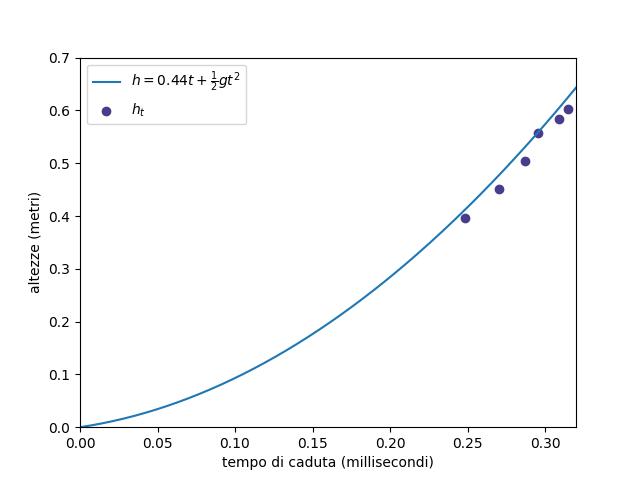
\includegraphics{relazione_caduta_libera/computed_data/parabola_corretta.png}
  		} %close resize
  	} %close centering
  	\caption{la funzione che descrive il fenomeno è stata corretta per \(v_{0}\neq 0\)}
\end{figure}

\noindent Correggiamo i dati per poter eseguire l'interpolazione lineare
\begin{figure}[!htbp]
	\captionsetup{labelformat=empty}
	\caption{Tabella2.b}
	\makebox[1 \textwidth][c]{ 
		\begin{tabular}{c|c}
			\hline
			\hline
			y: altezza-\(v_{0}\)t (m) & x: tempo di caduta\(^{2}\) (\(s^{2}\))\\
			\hline
			1: \(0.4639 \pm0.007\) &\(0.099\pm 0.001\)\\
			2:  \(0.4474 \pm   0.007\)& \(0.096 \pm 0.001\)\\
			3:  \( 0.4270 \pm 0.007\)& \(  0.087 \pm 0.002 \)\\
			4: \(0.3781 \pm  0.006\)& \(  0.083 \pm  0.001 \)\\
			5: \(0.3317 \pm0.006 \)&  \( 0.073 \pm  0.001\)\\
			6: \(  0.2865 \pm 0.005\) &\(0.062 \pm  0.001\)\\
			\hline
			\hline
		\end{tabular}
	} %close centering
	\caption{con \(v_{0} = 0.44 \pm 0.02 \frac{m}{s}\)}
\end{figure}

\noindent Notiamo che \(\sigma_{hi} >> \sigma_{ti}\), questa volta consideriamo trascurabile l'incertezza sui tempi al quadrato.

\[B_{corretto}=4.9 \pm 0.2 m/s^{s} \qquad A=-0.02  \pm 0.02 m\]
.\\\\\\\\\\\\\\
\begin{figure}[!ht]
	\captionsetup{labelformat=empty}
	\makebox[1 \textwidth][c]{       %centering table
		\resizebox{0.90 \textwidth}{!}{   %resize table
			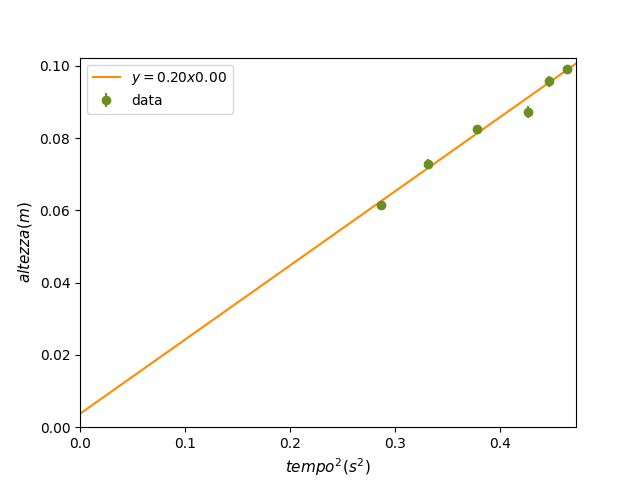
\includegraphics{relazione_caduta_libera/computed_data/retta_corretta.png}
		} %close resize
	} %close centering
\end{figure}

\noindent L'interpolazione dei dati che considerano una velocità iniziale diversa da 0 porta ad una stima per g pari a: \(9.759\pm 0.348 \frac{m}{s^{2}}\).  \( t= \frac{\left | g_{corretta} - g_{attesa} \right |}{\sigma_{g}} = 0.14\rightarrow\)  probabilità di  accuratezza: 89\(\%\). \\
\noindent L'errore sistematico commesso sulla prima stima per g è stimabile con: \(\left | g_{corretta} - g\right |=1.5 m/s^{2}\), decisamente non trascurabile.
\end{document}